\pagestyle{fancy}
\fancyhf{}
\renewcommand{\headrulewidth}{0pt}
\fancyfoot[C]{\leftmark}
\fancyhead[R]{\thepage}
\doublespacing
\chapter{Glassy binary mixture with large size bidispersity: interdiffusion}


%
\section{Introduction}
\label{sec1}
%
Many soft matter systems as well as many biological systems consist of particles of very different sizes \cite{bechinger2013, weiss2014, hoefling2013}. These systems may show a glassy dynamics with a time-scale separation of relaxation processes among the different constituents. Examples of such systems are glassforming mixtures of small and large particles that have been studied experimentally via various colloidal and organic systems \cite{imhof1995_1, imhof1995_2, kurita2010, blochowicz2012, bierwirth2018, sentjabrskaja2016, laurati2019} and numerically via hard or soft sphere systems in computer simulations \cite{moreno2006, horbach2009, xu2012, xu2015, lazaro2019} as well as in the framework of mode-coupling theory (MCT) \cite{bosse1987, bosse1995, voigtmann2011}. A common feature in these studies is a freezing of the large particles into a glass state while the small particles remain mobile.  Here, the dynamics of the small particles is typically associated with anomalous diffusion on long transient time scales, as reflected, e.g., by a sublinear growth of the mean-squared displacement $\delta r^2(t)$ as a function of time $t$, i.e.~$\delta r^2(t) \propto t^\alpha$ with $\alpha<1$. In computer simulations as well as experiments of disparate-sized mixtures \cite{kurita2010, blochowicz2012, horbach2009, schnyder2018, kurzidim2011}, one finds values for the exponent $\alpha$ that in general depend on the temperature, the total density of the system, the concentration of small mobile particles, and the interactions between the particle, especially those between the large and the small particles. Thus, {unlike the case of model systems such as the Lorentz gas \cite{hoefling2013, schnyder2018}}, the values of $\alpha$ are non-universal and there is typically the lack of a sharp critical point at which one observes an asymptotic subdiffusive behavior in the longtime limit with a universal value of the exponent $\alpha$.  This non-universal behavior can be due to the thermal motion of the particles or soft interactions between small and large particles.

In a binary mixture of small and large particles, there are the two corresponding selfdiffusion coefficients $D_{\rm s}$ and $D_{\rm l}$, respectively, that characterize on one hand the glassy dynamics of the large particles ($D_{\rm l}$) and on the other hand the transport of the mobile small particles ($D_{\rm s}$). However, in addition to these single-particle transport coefficients, there is also a collective diffusion coefficient, namely the interdiffusion coefficient $D_{\rm AB}$, that characterizes the mass transport in the binary mixture \cite{fitts1962, akcasu1997, horbach2007}. In good approximation, $D_{\rm AB}$ can be often expressed as a simple linear combination of the selfdiffusion coefficients,
%
\begin{equation}
D_{\rm AB} = \Phi \left( x_{\rm l} D_{\rm s} + x_{\rm s} D_{\rm l} \right), 
\label{eq_darken}
\end{equation}
%
with $x_{\rm l}$ and $x_{\rm s}$ the concentration of the large and the small particles, respectively, and $\Phi$ the thermodynamic factor (see below). Equation (\ref{eq_darken}) is often called  the Darken equation \cite{darken1949} or the Hartley-Crank equation \cite{hartley1949}.  Computer simulations of glassforming metallic systems Al-Ni and Zr-Ni with different compositions \cite{horbach2007, kuhn2014} have shown that Eq.~(\ref{eq_darken}) qualitatively reproduces the temperature dependence of the interdiffusion coefficient, especially at low temperatures.  

The question of whether the interdiffusion coefficient can be expressed in terms of the selfdiffusion coefficients has been extensively discussed in the literature, especially in the context of (binary) polymer mixtures \cite{akcasu1997, bearman1960, brochard1986, sillescu1987, akcasu1991, hess1990}.  In this context, Eq.~(\ref{eq_darken}) is often referred to as the result of a ``fast mode theory'' \cite{akcasu1997}, because according to Eq.~(\ref{eq_darken}) for a disparate-sized binary mixture the interdiffusion coefficient would be essentially given by the selfdiffusion coefficient, $D_{\rm s}$, of the fast mobile species.  In a ``slow mode theory'', however, the opposite behavior is predicted.  Here, the relation between the interdiffusion and the selfdiffusion coefficients is given by \cite{hess1990}
%
\begin{equation}
D_{\rm AB} = \frac{\Phi}{\frac{x_{\rm l}}{D_{\rm s}} + \frac{x_{\rm s}}{D_{\rm l}}}, 
\label{eq_slowm}
\end{equation}
%
This result can be obtained in the framework of a random phase approximation \cite{akcasu1997}.  It implies that in a disparate-sized mixture $D_{\rm AB}$ is dominated by the selfdiffusion coefficient of the slow species, $D_{\rm l}$.  Note that in the framework of MCT one also finds that $D_{\rm AB}$ tends to ``follow'' the slow species such that it always vanishes in a glass state \cite{latz1990}.

For our study, we consider an equimolar binary AB mixture of soft spheres for which the size ratio of the two species is $\approx 2.85$ and, in addition, the strength of the interaction between AB pairs is weaker than that between AA and BB pairs. In an earlier molecular dynamics (MD) simulation study of this system \cite{horbach2009}, it has been demonstrated that on the typical time scale accessible in the MD simulation the A species falls out-of-equilibrium around the MCT critical number density which is at $\rho_c = 2.23$, corresponding to a number density of A particles $\rho_{c}^{\rm A}=1.115$.  While the A species is in a frozen-in state above $\rho_c$, the B species remains mobile and there is a relatively weak decrease of the corresponding selfdiffusion coefficient $D_{\rm B}$ with increasing density above $\rho_c$. We demonstrate that Eq.~(\ref{eq_darken}) very well describes the  density dependence of the interdiffusion coefficients and thus at high density $D_{\rm AB}$ is proportional to $D_{\rm B}$. Note that in our discussion, we use the MCT critical number density as a reference to indicate the density regime beyond which the glassy regime lies. In reality, as is well known, the mode coupling transition is avoided. In this work, as discussed below, we try to provide an estimate of the glass transition density, viz. $\rho_g\approx{2.3}$.

We show that the approximative proportionality $D_{\rm AB} \propto D_{\rm B}$ is associated with strong finite-size effects of the selfdiffusion coefficient of the slow large species, $D_{\rm A}$. These finite-size effects are due to the relation of $D_{\rm AB}$ to the diffusion coefficient of the centre of mass of species $\alpha$ (with $\alpha = {\rm A, B}$), $D_{\rm cm}^{(\alpha)}$. Note that $D_{\rm cm}^{\rm (A)} = D_{\rm cm}^{\rm (B)}$ holds because the total system's centre of mass is fixed.  As we shall see below, $D_{\rm cm}^{\rm (A)} \propto D_{\rm AB}/N$, with $N$ the total number of particles in the system. Thus, the selfdiffusion coefficient of the A species, $D_{\rm A}$, has a finite-size correction $\propto D_{\rm AB}/N \propto D_{\rm B}/N$ that may be the dominant contribution to $D_{\rm A}$ for $\rho^{\rm A} \gtrsim \rho_{c}^{\rm A}$ and small system sizes. Only if one corrects the selfdiffusion coefficient $D_{\rm A}$ by computing it relative to the center of mass of the A species, one can extract the true value of $D_{\rm A}$ without the $1/N$ correction. As we argue below, similar features could be observed in any glassforming system with strong dynamic heterogeneities.  In such systems, there can be clusters of slow particles with a relatively fast center-of-mass motion on time scales where no particle rearrangements inside the cluster occur. Therefore, our study reveals a common feature in the dynamics of glassforming liquids.

The rest of the chapter is organized as follows: In Sec.~\ref{sec2}, we present the model of the AB mixture, the details of the simulation and quantities used to analyze the structure and dynamics of the system. The results of the analysis of structure and dynamics are given in Sec.~\ref{sec3}, followed by a summary and conclusions in Sec.~\ref{sec4}.   

%
\section{Model and methods}
\label{sec2}
%

%
\subsection{Interaction potential and details of the simulation}
%
The system that we study \cite{horbach2009} is a binary $50-50$ mixture of repulsive particles, where the diameter of the bigger particles (species A) is sampled from a uniform distribution, i.e.~$d_{\rm A} \in [0.85,1.15]$, while the diameter of the smaller particles (species B) is $d_{\rm B} = 0.35$ (see Fig.~\ref{fig6p1}). The average size ratio of A and B particles is $\langle d_{\rm A}\rangle/d_{\rm B} \approx 2.85$ where $\langle d_{\rm A}\rangle \approx 1$. A pair of particles $\{\alpha,\beta\}$ (with $\alpha = {\rm A, B}$ and $\beta = {\rm A, B}$), separated by a distance $r$, interacts via a Weeks-Chandler-Andersen (WCA) potential \cite{weeks1971}, i.e.~a Lennard-Jones potential that is cut off at its minimum and shifted to zero. To further smoothen the WCA potential, we also add a term that provides the continuity of its derivative. Thus, the potential is defined by 
%
\begin{eqnarray}
\textrm{V}_{\alpha\beta}(r) &=& u_{\alpha\beta}(r)-u_{\alpha\beta}(R_{c})-\left(r-R_{c}\right)\left.  \frac{du_{\alpha\beta}}{dr}\right|_{r=R_{c}},\nonumber\\
u_{\alpha\beta}(r) &=& 4\epsilon_{\alpha\beta}\left[\left(\sigma_{\alpha\beta}/r\right)^{12}- \left(\sigma_{\alpha\beta}/r\right)^{6}\right]\: ,
\end{eqnarray}
%
for $r<R_{c} = 2^{1/6} \sigma_{\alpha\beta}$, else $\textrm{V}_{\alpha\beta}(r) = 0$, with $\alpha, \beta$ as particle index. Here, $\sigma_{\alpha\beta} = (d_{\alpha}+d_{\beta})/2$ and $\epsilon_{\alpha\beta} = \epsilon = 1.0$ if both interacting particles are of the same type, else $\sigma_{\alpha\beta} = (1.00+0.35)/2$ and $\epsilon_{\alpha\beta} = 0.1$.  All particles have the same mass $m_{\rm A} = m_{\rm B} = m = 1$.  In the following, length, energy, and time are measured in units of $\langle d_{\rm A} \rangle$, $\epsilon$, and $\tau_{\rm WCA} = [m \langle d_{\rm A} \rangle ^2/\epsilon]^{1/2}$, respectively.

%%%%%%%%%
\begin{figure}
\centering
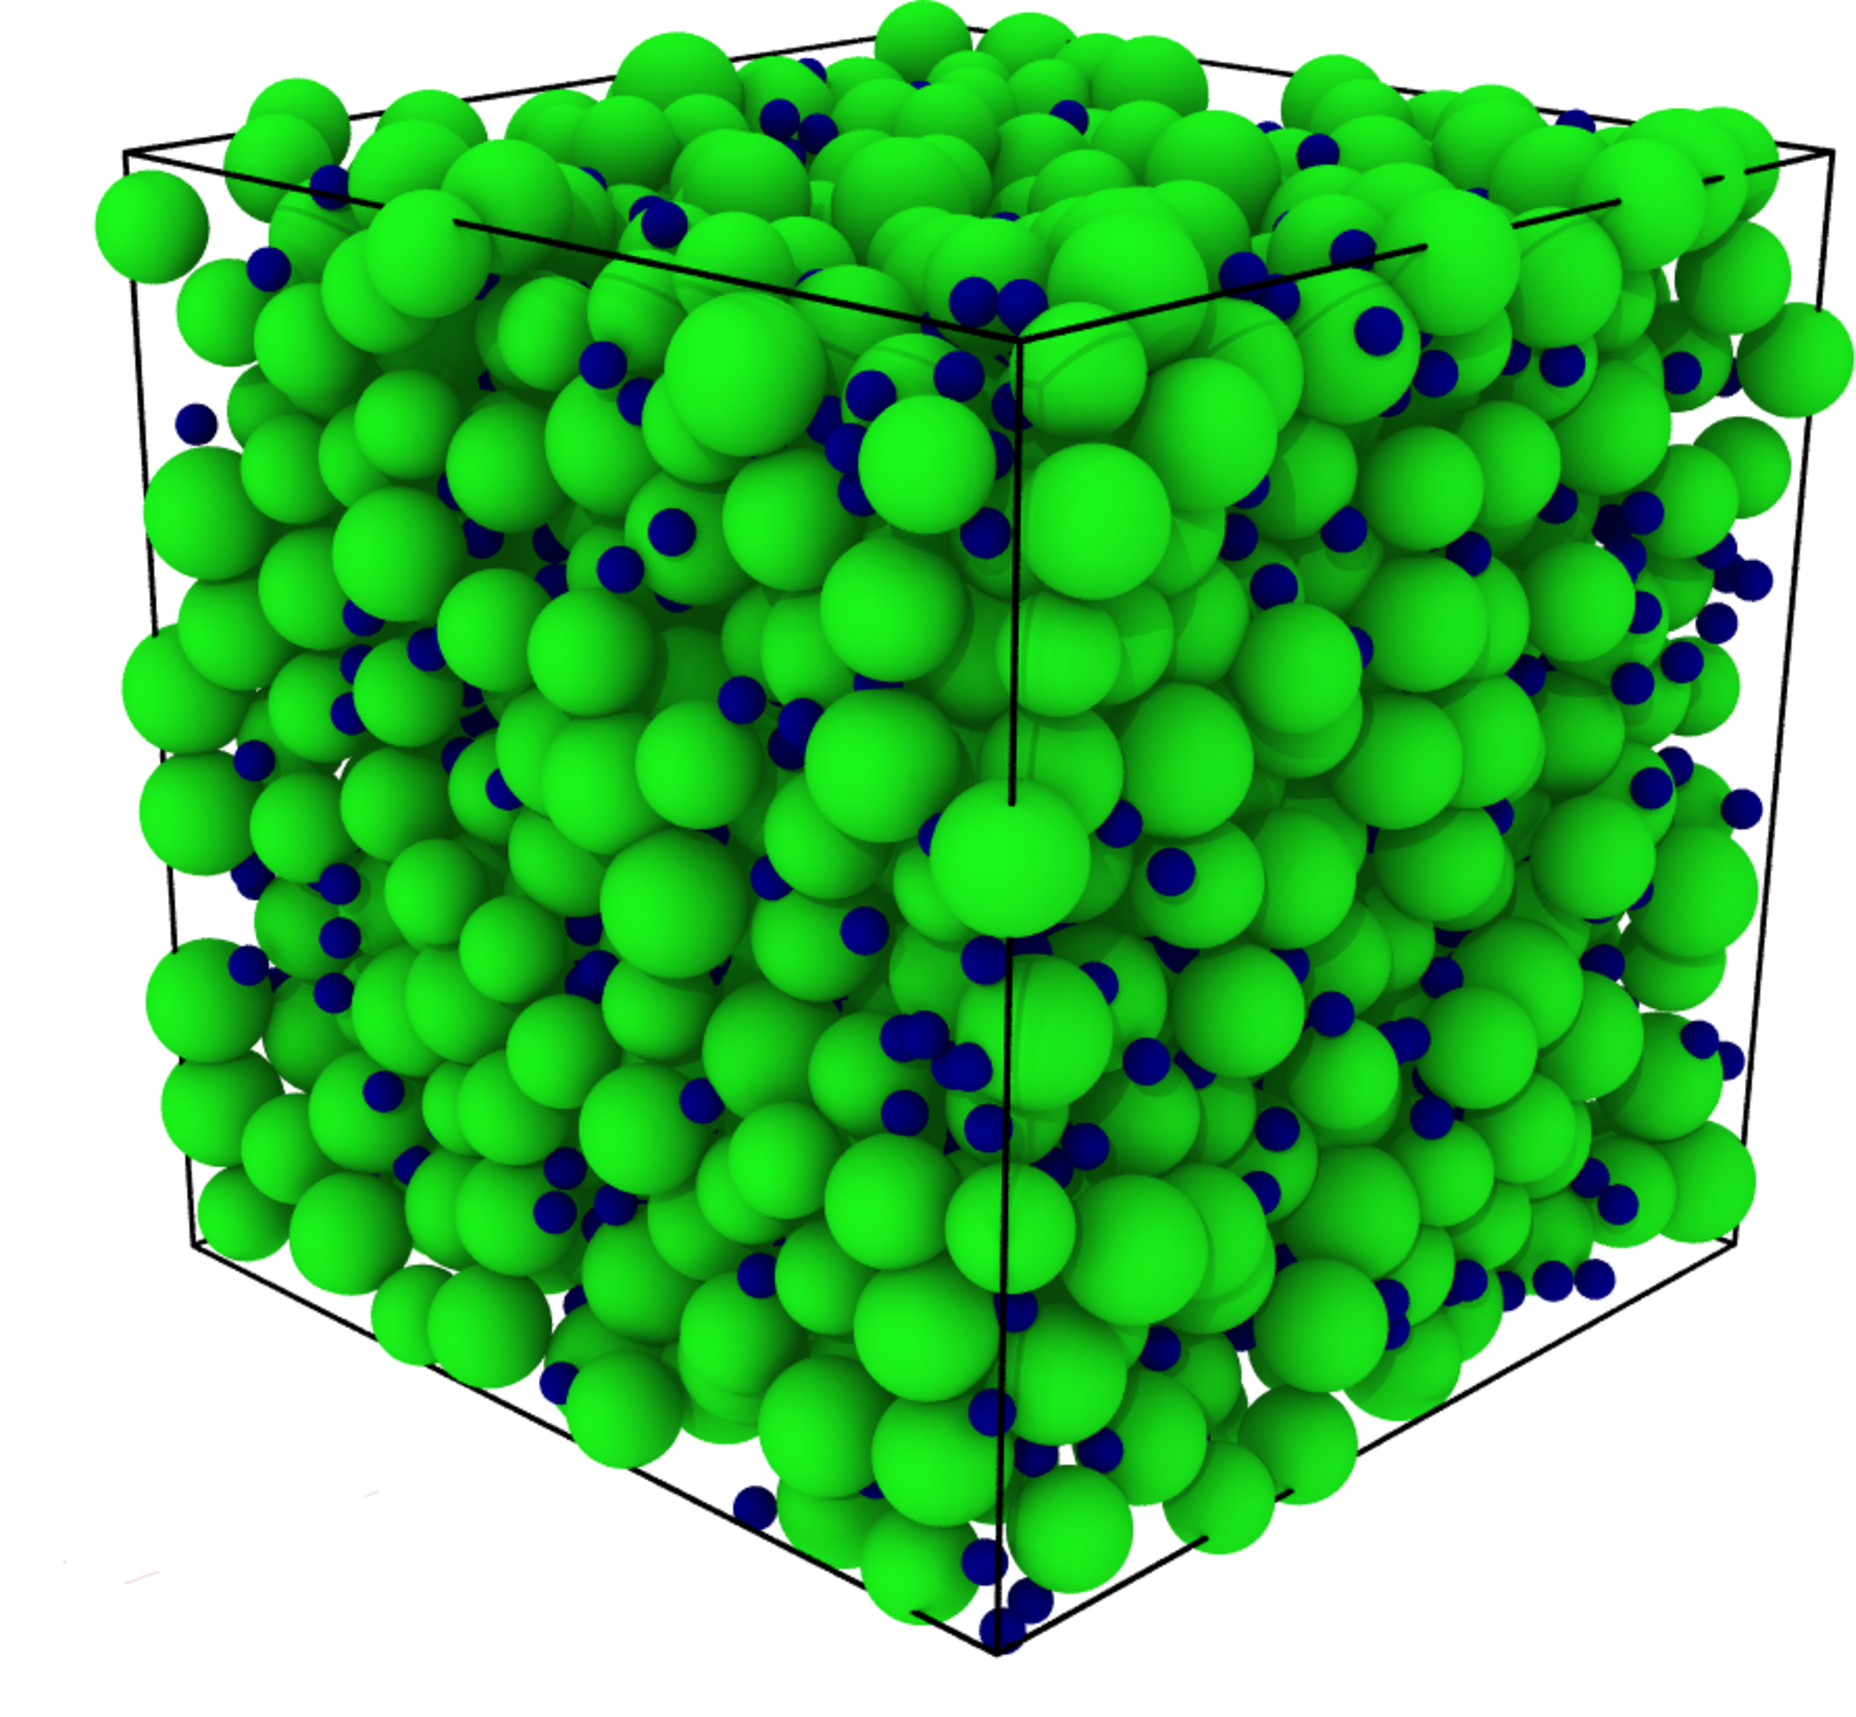
\includegraphics[width=12cm]{figs/fig6p1.pdf}
\caption{Snapshot of the system at the density $\rho = 2.5$. A and
B particles are represented by green and dark blue spheres, respectively.
\label{fig6p1}}
\end{figure}
%%%%%%%

Using LAMMPS \cite{plimpton1995}, extensive molecular dynamics (MD) simulations are performed for systems with $N = 1000$, 2000, and 4000 particles, placed in a three-dimensional cubic box with periodic boundary conditions. Except otherwise stated, all reported results are for $N=2000$. The equations of motion are integrated using the velocity form of the Verlet algorithm \cite{allen2017} with a time step $dt = 0.00075 \, \tau_{\rm WCA}$.  The simulations are done for different number densities in the range $2.1 \le \rho \le 3.5$ at the temperature $T = 2/3$. For each density, 30 independent samples are simulated.  During the equilibration of the samples, the temperature is kept constant using a dissipative particle dynamics (DPD) thermostat \cite{soddemann2003} where the damping coefficient is set to 1.0. {Note that the DPD thermostat conserves linear momentum locally and thereby globally. And, we have chosen the damping coefficient such that the short-time dynamics under thermostatted conditions matches with the dynamics reported under microcanonical conditions \cite{horbach2009}. Furthermore, to obtain well-annealed samples at} the high densities, $\rho \ge 2.25$, the MD simulations are combined with the swap Monte Carlo (SMC) algorithm \cite{grigera2001, berthier2019}.  In a trial SMC move, one randomly selects a pair of particles, exchanges their diameters, and accepts or rejects this move according to a Metropolis criterion. In our scheme, only the diameters of the A particles are swapped. Every 100 MD steps, $N_{\rm A}$ trial SMC moves are done. The runs with the hybrid MD-SMC method were over $4 \times 10^8$ time steps for $\rho = 2.25$ and $6 \times 10^8$ time steps for $\rho \ge 2.296$. This is sufficient to fully equilibrate the system up to a density of 2.296. This we have checked by analyzing the decay of the incoherent intermediate scattering function (see below) in the presence of the SMC. Thus, the glass transition in our simulation occurs around $\rho_{\rm g} \approx 2.3$. For the MD production runs, the SMC is switched off, but they are performed with the coupling to the thermostat.

A snapshot of the system at the density $\rho = 2.5$ is shown in Fig.~\ref{fig6p1}. From this snapshot, one can infer that the large A particles form a close-packed structure while the small B particles can explore the free volume between the A particles.



%
\section{Results}
\label{sec3}



%
\section{Summary and conclusions}
\label{sec4}
%
Our work elucidates several aspects of the diffusion dynamics in an equimolar glassforming binary soft-sphere mixture with large size ratio.  We observe a very pronounced time scale separation between the motion of the slow A species and that of the fast B species at high densities. As a consequence, the A particles show the typical glassy dynamics of a densely packed system, while the B particles remain mobile at very high densities, $\rho > \rho_c$, exploring the void space in between the A particles. We have seen that the interdiffusion coefficient $D_{\rm AB}$ can be well approximated by the Darken equation (\ref{eq_darken}).  Since at high density $D_{\rm A} \ll D_{\rm B}$, one therefore obtains $D_{\rm AB} \approx \Phi x_{\rm A} D_{\rm B}$, i.e.~the interdiffusion coefficient is dominated by the fast species.  For our equimolar mixture, we can also write $D_{\rm AB} = \Phi N D_{\rm A}^{\rm cm}$ and thus at high density we have $D_{\rm A}^{\rm cm} \approx D_{\rm B}/(2N)$.  This implies that even if the A particles form a frozen-in structure with essentially no rearrangements of the relative positions of particles, they may follow collectively the diffusive motion of their center of mass and one finds for the selfdiffusion coefficient $D_{\rm A} \approx D_{\rm A}^{\rm cm} \propto N^{-1}$. One can, of course, correct for this finite-size effect by computing one-particle quantities such as MSD$_{\rm A}(t)$ and $F_s^{\rm A}(q,t)$ from the center-of-mass-corrected coordinates, as defined by Eq.~(\ref{eq_rprime}).

The finite-size effects, that we have reported in this work with respect to the selfdiffusion coefficient of the slow species, are expected to be a typical feature in glassforming binary mixtures with large size ratio. Moreover, one may expect similar effects in any glassforming system with strong dynamic heterogeneities. {Furthermore, studying interdiffusion dynamics with changing composition as well as size-ratio of the mixture would be of interest, since variation of these parameters are known to change extensively the dynamical properties of the mixture \cite{zac2005, vinaySoft}}.

{Finally, we note here that the rectification process elucidated in this work to obtain the correct dynamical behaviour is not only relevant for quiescent systems, but also in the case where such mixtures are externally driven, e.g. under shear \cite{vinay}. }
%


\section{Outlook}
Different studies performed in this thesis under the title "{\em Thermo-mechanical response of glassy systems}" can be extended in many directions, leading to some interesting results. Let's discuss some possible project which can be continued as a follow up of this thesis.

\begin{itemize}
    \item {\bf \em Thermal response of network glass-formers and polymeric glasses:} In this thesis in Chapter-\ref{chap3}, we have studied the response of a glass-forming system to a thermal gradient. But the model glass-former that we have used is non-bonded and non-network forming. Therefore, a possible extension of the project to glass-forming systems that form network, due to special transport properties of these systems. An example of such glass-former is silica, which is common to many applications. Also, heat transport process can be studied in polymeric glassy systems.
    
    \item {\bf \em Influence of temperature gradient in the immobilization of nuclear waste in glasses:} Borosilicate and phosphate glasses are, in general, used for radioactive nuclear waste immobilization. In this process, because of high temperature of waste material, there is a chance of leakage of radioactive isotopes because of Soret migration. This type of phenomenon is very poorly studied. Extending our project in Chapter-\ref{chap3} to such studies can be very helpful.
    
    \item {\bf \em Thermal response in granular system:} The study that we have performed in Chapter-\ref{chap3} in the context of glassy systems, can be extended to granular systems like concrete. Some granular materials are used as heavy duty material where one part of the material becomes very hot while the inner part of the material being cold. Now, it becomes very important to understand the role of such temperature gradients in crack formation in granular solids.
    
    \item {\bf \em Designing speciality heterogeneous glassy materials via thermal protocol:} The idea developed in Chater-\ref{chap3} to design inhomogeneous glassy materials using a temperature gradient pulse, can be further developed to design a material with specific type of inhomogeneity such that the pathway of mechanical failure could be controlled, something similar to shown in Chapter-\ref{chap4}.
    
    \item {\bf \em Compression and expansion studies on inhomogeneous glasses obtained via thermal processing:} We have studied the shear response of inhomogeneous glasses obtained via thermal processing in Chapter-\ref{chap4}. This project can be extended to study compression and expansion protocols of deformation in the context of inhomogeneous glasses that we have prepared. Such deformation protocol can lead to more insights to the failure in hetrogeneous glassy materials.
    
    \item {\bf \em Impact of thermal cycling on mechanical properties of glasses:} In Chapter-\ref{chap4}, we used a temperature gradient pulse to prepare inhomogeneous glassy samples. We can cyclically apply and remove the thermal gradient to create a thermal cycling process. The thermal and mechanical properties of glasses are expected to show some interesting properties under such thermal cycling.
    
    \item {\bf \em Mechanical response of inhomogeneous glassy materials prepared via local annealing:} Using the recently developed SWAP Monte-Carlo (also discussed in section-\ref{swap} in Chapter-\ref{chap2}) techniques, we can do local annealing of the material to prepare a glassy sample with spatially inhomogeneous stability. The shear-deformation studies of these materials can help us in getting insights to failure mechanism at microscopic level.
    
    \item {\bf \em Poiseuille flow with temperature gradient: } The Poiseuille flow study that we have performed in Chapter-\ref{chap5} where the temperature of the flowing liquid can be controlled via a vibrating wall, can be extended to study a channel flow where both the walls are maintained at slightly different temperatures. Understanding the flow behaviour in such setup with confining wall at different temperatures can be useful for many practical applications.
    
    \item {\bf \em Couette flow of glassy liquid with thermal control via walls:} It would be very interesting to explore Couette flow of glassy liquid in a set-up where temperature is controlled via walls, very similar to thermal control that we have used in chapter-\ref{chap5}. This can lead to some non-trivial flow behaviour in comparison to Couette flow set-up where temperature of confining fluid is directly controlled.
    
    \item {\bf \em Jamming scenario in the context of binary mixture with large size bidispersity:} In Chapter-\ref{chap6}, we have studied interdiffusion and rheological properties of a binary mixture where the size ratio between bigger and smaller species is relatively larger than the conventional mixtures. The athermal rheology of such mixtures is not well studied, which could be possible extension to our work in Chapter-\ref{chap6}.
    
    \item {\bf \em Rheological response of glass-forming systems with medium range crystalline order:} A class of glass-formers in two dimensions show medium range crystalline order, with crystalline patches which grow as glass transition is approached. It would be a very interesting project to explore the shear response of such materials to understand the impact on crystalline order.
\end{itemize}
